\chapter{\label{chap:introduction}Introduction}

%intro to title and topic (start broad and work down to more detail. Try to captivate the reader)
For decades the idea of re-usable software has been seen as the holy grail of software development. Even in the eighties, papers were already written about this topic~\cite{standish1984essay}. Throughout the years, more and more research has been done on the benefit of re-usable software~\cite{jacobson1997software}. Studies have also been performed on how to re-use software in practice~\cite{reifer1997practical}. But up until recently, there was more discussion about software re-use than actual software re-use. Even though most software uses the same blocks of code over and over again, almost all software is built from the ground up~\cite{frakes2005software}. Today, this situation is completely different. Nowadays, almost every application re-uses software in the form of software dependencies. However, this re-use pattern is starting to become unchecked. The shift to re-usable software has happened so quickly, the risks associated with choosing the right dependencies are often overlooked~\cite{cox2019surviving}. 

%Describe the topic and scope of your research
\section{Code Evolution}
% Monolithic and libraries
Over the years, the way we use code has evolved with the changing need of the users and society as a whole~\cite{rajlich2014software}. This evolution started with specific applications written for each use case and each platform it had to run on. These so called monolithic applications took extensive amounts of time to develop and could not be re-used.

\begin{figure*}[th!]
	\centering
	\begin{subfigure}[t]{.45\textwidth}
		\centering
		\captionsetup{width=.9\linewidth}
		{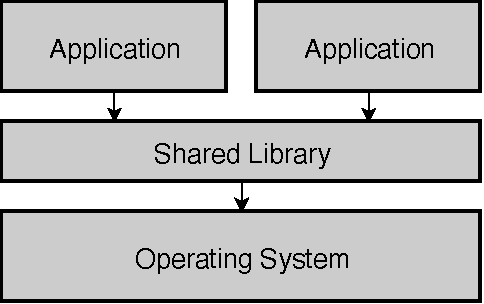
\includegraphics[width=0.77\linewidth]{images/intro-evolution-shared-library2.pdf}}
		\caption{Shared Library.}
		\label{fig:shared-library}
	\end{subfigure}\hfill%
	\begin{subfigure}[t]{.55\textwidth}
		\centering
		\captionsetup{width=.9\linewidth}
		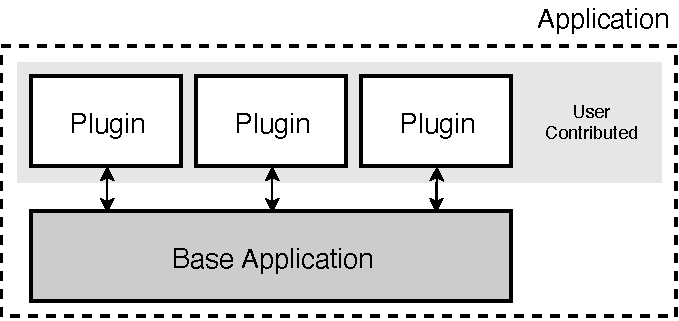
\includegraphics[width=0.97\linewidth]{images/intro-evolution-plugin2.pdf}
		\caption{Plugin Architecture.}
		\label{fig:plugin}
	\end{subfigure}\vspace{0.5cm}\hfill%
	\begin{subfigure}[t]{.45\textwidth}
		\centering
		\captionsetup{width=.9\linewidth}
		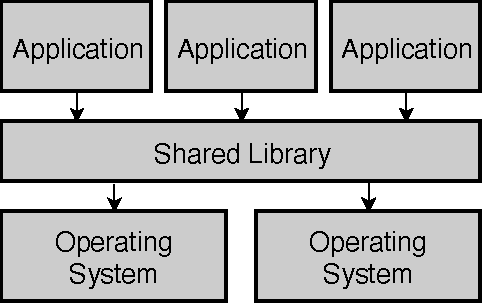
\includegraphics[width=0.77\linewidth]{images/intro-evolution-cross-platform2.pdf}
		\caption{Cross-platform Application.}
		\label{fig:cross-platform}
	\end{subfigure}%
    \begin{subfigure}[t]{.55\textwidth}
    	\centering
    	\captionsetup{width=.9\linewidth}
    	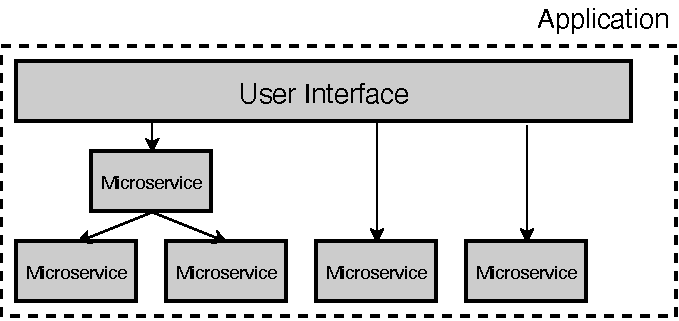
\includegraphics[width=0.97\linewidth]{images/intro-evolution-microservice2.pdf}
    	\caption{Microservice Architecture.}
    	\label{fig:microservice}
    \end{subfigure}%
	\caption{Architectures in the evolution of software.}
	\label{fig:evolution}
\end{figure*}

\newpage

To reduce this time, system libraries were built to make it possible to run these applications on similar platforms. A visualization of this architecture can be seen in Figure~\ref{fig:shared-library}. This abstraction layer, however, was still limited to broader types of platforms e.g. Linux, Unix, Windows. These shared system libraries could now be maintained and distributed separately. This led to easier development and applications that could be used on more systems.

% Example
A good example of this evolution is the Debian package system. It made it possible for code that was meant to be used as a library to be packaged separately for both system and user code. This allowed applications to indicate which library would be required for that application and the system would make sure it is available to the application. This possibility allowed these applications to be developed faster. ~\cite{zacchiroli2011debian}

% Plug-ins
% In computing, a plug-in (or plugin, add-in, addin, add-on, or addon) is a software component that adds a specific feature to an existing computer program. When a program supports plug-ins, it enables customization. to enable third-party developers to create abilities which extend an application, to support easily adding new features, to reduce the size of an application, to separate source code from an application because of incompatible software licenses.

These new shared code libraries provided numerous benefits and speed to application developers, but to improve the ecosystem further a new step had to be made. At this point when applications were distributed they were static. There was no option to adapt the application to include features that the user would like to see. Also, users that wanted to add their own functionality had to go through the developers to accomplish this. To solve this, the larger applications began to include plug-in systems. A visualization of this architecture can be seen in Figure~\ref{fig:plugin}. A plug-in system allows specific functionality to be added to an existing computer program. This enabled customization of applications, making it possible to reduce the size of the core application or separating source code because of incompatible licenses. This paradigm allowed the rapid development of extra features by both developers and the users of the application.

% Example
A well-known example of a program with a plugin system is Winamp. The Winamp developers used a plug-in system to provide users with a customizable package that could serve each user's preference~\cite{nullsoft1999winamp}. A large community formed around the application with different plug-ins for every imaginable feature~\cite{winampcommunity}. This community-building gave an incentive for other applications to implement similar plug-in systems.

% Cross-platform applications
% software written in an interpreted language or pre-compiled portable bytecode for which the interpreters or run-time packages are common or standard components of all platforms
Eventually, programming languages were created that allowed the development of cross-platform applications that could be run on all common platforms. This eliminated the need to create separate binaries for each individual platform. These applications were either written in an interpreted language, e.g. Python, or in a pre-compiled portable byte-code format for which interpreters exist on all platforms, e.g. Java. A visualization of this architecture can be seen in Figure~\ref{fig:cross-platform}. In the last decade, a major part of these cross-platform applications has moved towards the web. These new web applications make use of existing cross-compatibility of web technologies, that were designed when the web became universal, that run on all platforms.

%  Code frameworks e.g. Spring, Wordpress, Android
With the development of cross-platform applications, there was also a rise in the availability of code frameworks. A code framework provides particular functionality as part of a larger software platform to facilitate the development of software applications. Software with common use-cases could make use of the abstraction provided by these code frameworks to create application-specific software with only limited additional user-written code. These code frameworks can be seen everywhere nowadays. Some examples of code frameworks are Spring, WordPress, and the Android platform. Spring is a popular code framework for developing applications in Java. WordPress is a web framework that runs more than 25\% of the websites on the internet~\cite{ewer201414}. The Android platform is the underlying framework that allows apps to be created for the Android mobile operating system.

% Micro-services
% collection of loosely coupled services
A more recent concept in the development of software applications is the microservice architecture. This architecture breaks an application up into a collection of loosely coupled services. These services are normally small in size and have one use-case that they were specifically designed for~\cite{thones2015microservices}. The microservice architecture facilitates code re-use on a big scale with platforms like NPM (Node Package Manager) storing over 750.000 JavaScript packages~\cite{npmstatistics}. A visualization of this architecture can be seen in Figure~\ref{fig:microservice}.

\section{Code Re-use}

The constant factor during this code evolution is code re-use. The ability to make development easier and faster by making use of existing solutions already created by a different party.

% We want re-use so badly, yet our failures are spectacular. Almost all major technology trends of the past 20 years touts reuse as the saving grace. Vendors have sold billions of dollars in software through the broken promise of increased reusability. https://dzone.com/articles/reuse-dream-dead
Re-use is software development’s unattainable goal. The ability to put together systems from re-usable elements has long been the ultimate dream. Almost all major software design patterns resolve around extensibility and re-use. Even the majority of architectural trends aim for this concept. Despite many attempts in almost every community, projects using this approach often fail~\cite{reusedreamdead}.
%In general, the more reusable we choose to make a software component, the more difficult that same software component is to use. In the extreme, an infinitely reusable component is infinitely difficult to use. Dealing with the tension between re-use and use is a complex issue, and often, we fail. Largely, the problem has to do with dependencies.
This is attributed to one big problem: usability. The more reusable we try to make a software component, the more difficult it becomes to work with said component. This is a critical balance that needs to be worked on.

\subsection{Re-usability vs Usability}
%The challenge we run into when attempting to create a highly reusable component is to manage the tension between reusability and useability. In our example above, breaking out the coarse-grained component into fine-grained components makes it more difficult to use each of the resulting fine-grained components. Likewise, creating a lightweight component makes using the component more difficult since the component must be configured each time the component is used.
%
%Fine-grained components have more component dependencies and lightweight components have more context dependencies. Each makes a component more re-usable, but also more difficult to use. The key is to strike a balance, and that is a topic for another day not too far away.

The challenge we face when creating a highly re-usable component is to find this balance between re-usability and usability.

To make a component more re-usable it needs to be broken down in smaller parts, that each handles only one task. Components with multiple tasks are harder to re-use since each application has different use cases and therefore has to modify and maintain their own version of that component. Smaller components that handle only one task can be used as building blocks for bigger components making them easier to re-use, saving developers the need for maintaining their own version. However, to create complex application hundreds of small re-usable components would have to be used creating a problem of its own. How are all these components going to be managed? The largest part of this problem has to do with dependencies~\cite{reusedreamdead}, an additional piece of code a programmer wants to call. Some aspects to consider are:
\begin{itemize}
	\item Is the API (Application Programming Interface) going to stay constant?
	\item How do we deal with breaking changes?
	\item How do we prevent dependency conflicts?
\end{itemize}

\noindent Some of these aspects are already partly being addressed through Semantic Versioning~\cite{preston2013semantic}, but most of these are still unsolved today.

The context dependability of a component also greatly affects the balance between re-usability and usability. When a component depends on the context it is running in, it makes it impossible to move it to an different environment that does not have this context. For components to be more re-usable, this context has to be moved from code to configuration. However, if each small component has to be configured each time it is used, the application would become less usable.

Both the granularity and the degree of dependability on the context can improve the re-usability at the cost of usability. The key is to find a balance (Figure~\ref{fig:balance-scale}). 

\vspace{0.5cm}

\begin{figure}[h]
	\centering
	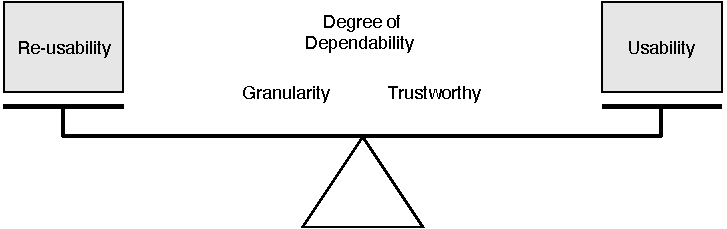
\includegraphics[width=0.9\textwidth]{images/intro-balance-scale.pdf}
	\caption{\label{fig:balance-scale} Balancing Re-usability and Usability.}
\end{figure}

\newpage

\section{Component Terminology} % Modules vs Plug-ins

Two different kinds of reusable components that are often integrated into applications are modules and plug-ins. Since these terms can have a different meaning depending on the application, the interpretation that this work will use is defined below:

\begin{itemize}
	\item \textbf{Modules} are main functionality components that are used to break up the application into smaller subsystems that can more easily be worked on with different/larger teams. Modules can either by re-usable components or tied to the specific application, and should be able to operate independently
	\item 
	% Plug-ins depend on the services provided by the host application and do not usually work by themselves. Conversely, the host application operates independently of the plug-ins, making it possible for end-users to add and update plug-ins dynamically without needing to make changes to the host application
	\textbf{Plug-ins} are components used to extend the main functionality of the application without having to make changes to it. They are often created by the community of the application. The functionality in these plug-ins are often too small or too unique to integrate into the core application. Plug-ins depend on the services provided by the application, they do not operate independently. They are also tied to a specific application and can not be re-used for other applications.
\end{itemize}

\noindent The function of both kinds of components is, however, not different. They both provide extra functionality to the application. It would therefore also make sense to both make them first-class citizens of the application instead of making plug-ins a secondary operator.

This distinction is often made to differentiate between the code of the original authors and code created by third-parties. Plug-ins are most of the time also not reviewed by the original authors of the project.

% https://student.unsw.edu.au/introductions
\section{Research Goal}

% What is done, what is missing?
Over the last couple decades, extensive research has been performed into the field of software re-use. In this period, several survey studies have been done to see what different approaches were used in research literature for creating re-usable software~\cite{krueger1992software}~\cite{frakes2005software}. The surveys tried to make generalizations about the methods used to research if there is a common pattern among them. The approaches mostly centered around re-using code for common use-cases like code frameworks. 

Other studies have worked on designing metrics and models for measuring progress in software re-use to identify the most effective strategies~\cite{frakes1996software}. Morisio et al looked at success and failure factors in software re-use to identify key factors in its adoption~\cite{morisio2002success}. The main cause of failures that they discovered was a lack of commitment by companies and projects.

%Normalized System theory == purist, holy grain and therefore inefficiency beyond usage. Too complex. 

A more recent study, attempted to build a framework for highly modular and extendable software systems, called Normalized System theory. This theory is based on a theoretical concept called system theory. This theory, however, takes the abstraction of modules to a level that makes it inefficient beyond usage. It takes this approach to make the system more agile. However, without simplicity all agility is lost. ~\cite{de2018enabling}

Lehman's laws of software evolution is a law describing the evolution of software. The law describes a balance between forces driving new developments on one hand, and forces that slow down progress on the other hand~\cite{lehman1980programs}~\cite{lehman1997metrics}~\cite{herraiz2013evolution}. One of the forces that slows down the progress of new developments is the ability of developers using the development to understand and easily use the functionality of the development.

%This framework attempts to solve the problems that exist in the software practices of today. One of these software practices is the microservice architecture. This architecture like explained in the introduction breaks an application up into a collection of loosely coupled services.

 Studies have been done into the practical issues that the microservice architecture creates when used in a software application~\cite{dragoni2017microservices}. Examples of these issues are the manageability of packages on NPM, no explicit dependencies, interfaces that are not well defined. The architecture makes use of completely decoupled services that communicate through REST APIs. This interface, however, limits the type of communication that can be send between the nodes. Newman et al concludes in a different study that the microservice architecture was specifically designed for maximizing re-usability without taking into account usability~\cite{newman2015building}.

Smart contracts, in particular Ethereum, is another software practice used today to solve the problem of code re-usability. However, since Ethereum is based on a proof-of-work principle, it requires payment so execute actions on the system. This will make applications build on top of Ethereum subject to these charges. In many cases these charges will have the consequence that the application would be to expensive to use in practice. The Ethereum model is not long-term sustainable
%Euthereum (smart contracts)
%https://medium.com/moatcoin/eth-gas-26d221c5c4c2
%IPv8 runtime model versus Ethereum fundamental brokenness (e.g. scalability and cost). :
%Back in October’17, an investor sent 1,700 ETH to a contract (AirSwapDEX) with a gas price
%of 400,000 Gwei and gas limit of 592,379. The Tx failed for some odd reason but the
%investor was charged whopping 236 ETH (\$122,086 as per today’s price)
%"Trustchain does not have a native cybercurrency such as Ethereum, it provides a transaction recording ledger". 
%cite: https://medium.com/moatcoin/eth-gas-26d221c5c4c2

\newpage

\subsection{Research Aim}

%Explain the scientific situation related to your topic - you can include the most important scientific articles and briefly explain them and how they are related to your research. 
% Discuss current situation/gap, explain why further research is necessary
% why (personal interest and interest for general use)
% - Another attempt at holy Grail of software re-usability

In the current research there exits a gap in balance between re-usability and usability. This works tries to fill that gap. People have tried solving the problem of software re-use, but it has proven to be a hard problem. There needs to be a trade-off between re-usability and usability.

This thesis focuses its work on developing a framework that continues the progression in the development of re-usable code. It tries to find a balance between the software practices of Today and the impractical concepts of the future.

There have already been many attempts to solve the goal of practical code re-usability. However, these attempts still left some problems open, that this thesis tries to solve. These problems include:

\begin{itemize}
	\item How to find a trade-off between re-usability and usability?
	%\item How to minimize the risk associated with the use of dependencies?
	\item Can we use social trust and crowdsourcing to improve security of libraries?
	\item How to ensure dependency availability efficiently and securely?
	% includes updates, trustability
	% NPM packages were deleted, but a lot of applications depended on this dependency
\end{itemize}

%contribution to the field (aim/goal)

\subsection{Research Scope}

% reiterate research aim
% Questions really broad, so scope should be limited
% Requirements zijn scope

 In the field of software engineering the concept of reusable software is a big topic. Tackling and solving a substantial problem like the trade-off between re-usability and usability is not feasible within a Master thesis project. Therefore this work limits the scope of the project to a subset of this problem. This subset consists out of the re-usability of applications that can be broken down into generalized modules defined by this work (which can be found in Chapter~\ref{chap:design}). This thesis will not provide a solution for every possible application type or applications with extreme complexity.

Within this subset, this work will propose one concept in the form of a framework to tackle the remaining research aims of trustworthiness and dependability on external components. The theoretical and practical properties of the framework are examined on the effectiveness of the discovery protocol and the module communication. Furthermore, one non-trivial use-case is used to determine that the concept works and is viable. 

% code library dependencies

\subsection{Research Structure}

%how (structure/method of the research) / methodology

Figure~\ref{fig:reading-guide} shows how the research is structured. The background and related work (Chapter~\ref{chap:introduction}) form the requirements which are specified in Chapter~\ref{chap:requirements}. These requirements are used as the underlying principles of the proposed concept, called FBase, explained in Chapter~\ref{chap:design}. A proof-of-concept implementation will be created to support the evaluation of the concept. The details of the implementation will be discussed in Chapter~\ref{chap:implementation}. Chapter~\ref{chap:evaluation} will analyze the concept with a non-trivial use-case. Based on the evaluation a conclusion will be given in Chapter~\ref{chap:conclusion}. 

%The rest of this document is outlined as follows: Chapter 2 will go further into the problems that this thesis tries to solve. Chapter 3 will discuss the solution proposed to solve the problems mentioned in Chapter 2. Chapter 4 will discuss the proof-of-concept implementation. Chapter 5 will evaluate the proposed framework against existing solutions. We use a concrete use-case driven methodology to advance the cause of software re-usability. 

\vspace{0.1cm}

\begin{figure}[h]
	\centering
	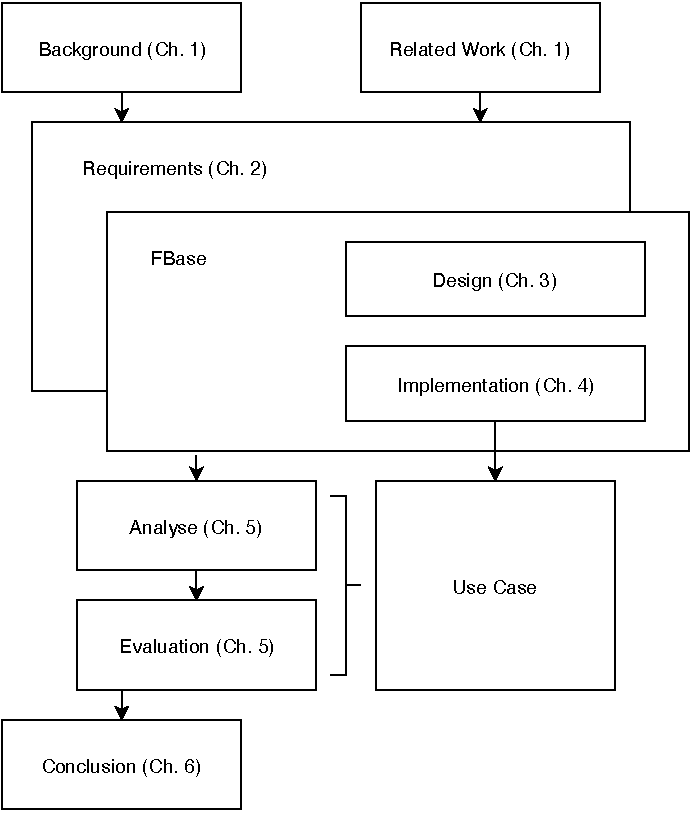
\includegraphics[width=1\textwidth]{images/intro-reading-guide.pdf}
	\caption{\label{fig:reading-guide} Research structure.}
\end{figure}
